\documentclass[11pt, oneside]{article}   	% use "amsart" instead of "article" for AMSLaTeX format
\usepackage{geometry}                		% See geometry.pdf to learn the layout options. There are lots.
\geometry{letterpaper}                   		% ... or a4paper or a5paper or ... 
%\geometry{landscape}                		% Activate for rotated page geometry
%\usepackage[parfill]{parskip}    		% Activate to begin paragraphs with an empty line rather than an indent
\usepackage{graphicx}				% Use pdf, png, jpg, or eps§ with pdflatex; use eps in DVI mode
								% TeX will automatically convert eps --> pdf in pdflatex		


%SetFonts

%SetFonts
%\usepackage{tikz}
%\usepackage{amsmath}	
%\usepackage{amssymb}
%\usepackage{xcolor}
%\usepackage{url}

%\usepackage[official]{eurosym}
%\usepackage{multicol}
%\usepackage{wasysym}

%\usepackage{academicons}
%\usepackage{dtklogos}
%\usepackage{braket}
%\usepackage{bm}
%\usepackage[utf8x]{inputenc}
%\usepackage{natbib}
\usepackage{multicol}
\usepackage{graphicx}
\usepackage{amssymb}
\usepackage{amsmath}
\usepackage{braket}
\usepackage{tikz}
\usepackage{pgfplots}
\pgfplotsset{compat=1.10}
\usepackage{filecontents}
%\usepackage{hyperref}
\usepackage{url}
\usepackage[makeroom]{cancel}
\usepackage{turnstile}
\usepackage[hypcap]{caption}
\usetikzlibrary{bayesnet}
\usetikzlibrary{positioning, arrows, decorations.markings, matrix, decorations}
\newcommand{\peh}{P(E|H)}
\newcommand{\phe}{P(H|E)}
\newcommand{\ph}{P(H)}
\newcommand{\pe}{P(E)}
\def\ci{\perp\!\!\!\perp}
\usepackage{amsthm}
\usepackage{bussproofs}
\EnableBpAbbreviations
\newcommand{\seq}{\Rightarrow}
\newcommand{\imp}{\rightarrow}
\newcommand{\bico}{\leftrightarrow}
\newcommand{\RLab}{\RightLabel}
\newcommand{\LLab}{\LeftLabel}
\newcommand{\logicname}{QMC}
\newcommand{\qax}{\ket{0} \seq}
\newcommand{\hadz}{\frac{1}{\sqrt{2}}\ket{0} + \frac{1}{\sqrt{2}}\ket{1}}
%\usetikzlibrary{positioning,arrows,decorations}
\usepackage{relsize}
%\usepackage[greek]{babel}
%\usepackage{amsfonts}
%\usepackage[utf8x]{inputenc}


\usetikzlibrary{bayesnet}
\usetikzlibrary{arrows, decorations.markings, matrix, decorations.pathmorphing}
\usetikzlibrary{decorations.pathreplacing}

\DeclareMathOperator{\graphrightarrow}{\tikz[baseline=-0.8ex]{ \draw [scale=1,->] (0,0) -- (4ex,0); }}
	\DeclareMathOperator{\graphleftarrow}{\tikz[baseline=-0.8ex]{ \draw [scale=1,<-] (0,0) -- (4ex,0); }}
	\DeclareMathOperator{\graphcontour}{\tikz[baseline=-0.8ex]{ \draw [scale=1,-] (0,0) -- (3ex,0); }}

	\DeclareMathAlphabet{\mathpzc}{OT1}{pzc}{m}{it}

\newenvironment{definition}[1][Definition]{\begin{trivlist}
\item[\hskip \labelsep {\bfseries #1}]}{\end{trivlist}}









\usepackage{mathrsfs}
\usepackage{lmodern}
\usepackage[T1]{fontenc} % Output font encoding for international characters
%\usepackage{natbib}










\sloppy
%\newtheorem{definition}{Definition}
\newtheorem{theorem}{Definition}


\usepackage{hyperref}
\usepackage{fontawesome5}
\usepackage[natbibapa,nodoi]{apacite}



\hypersetup{
    colorlinks = true,
    %linkbordercolor = {blue},
    linkcolor = {black},
    urlcolor = {blue},
    urlbordercolor = {blue},
    citecolor = {blue},
}

%\newtheorem{theorem}{Definition}

\setcounter{secnumdepth}{-2}

\title{Generative AI and Scientific Discovery: \\ Research Plan and Experience}
\author{Cameron Beebe, Ph.D.}
%\date{}							% Activate to display a given date or no date

\begin{document}
\maketitle
%\section{}
%\subsection{}




Assessing the limitations and risks from generative models used for scientific discovery, I focus on three areas: \textbf{i)} innovation of novel generative architectures; \textbf{ii)} responsible individual use of generative models; \textbf{iii)} how networks of scientists use generative models for discovery. This document includes a brief outlines the research area I would like to work on, lays out a methodology, provides writing samples, and summarises my relevant background for the project.

%This research plan proposes to philosophically address and contextualize the current (and perhaps future) capability of generative artificial intelligence with respect to scientific discovery.  

%In particular,   Following the brief outline of the topics I will work on, I also lay out a proposed methodology and summarize my background which is suitable for successful research and publication on this topic.

%I begin by introducing recent ideas from Atoosa Kasirzadeh on accumulative risk as a starting point for conceptualizing the current state of AI in our civilization using complex systems theory.  I agree with her arguments, and consider that at the level of the individual, as well as the sub-systems of scientific networks, are the components of the global complex system most crucial to avoid accumulative risk in.  





%\noindent This document provides a brief overview of my research experience and associated projects in AI, both practical and theoretical.  I have emphasized where relevant to reinforcement learning and explanation.  I have attached some excerpts from my written work and some brief commentary where appropriate to explain technical points.  The full context is available in online repositories of my projects,  papers, and dissertation.  


\tableofcontents








\section{Limits and Risks of Generative Scientific Discovery}


Generative machine learning models, when used in certain ways, have been demonstrated to produce non-trivial new scientific knowledge.  Are there limits to such knowledge? What risks, if any, might the particular use of generative tools in the context of discovery pose to the scientific method?  To begin to answer these questions I will consider three relevant aspects of generative models and their use in science:  \textbf{i)} innovation in generative model architectures used for discovery; \textbf{ii)} responsible individual use of generative models; \textbf{iii)} how networks of scientists use generative models for scientific discovery.  \\


%If new theories are generated, what status should they be afforded?  How would we explain a scientific discovery which was produced by a generative model?



%\noindent\textbf{Philosophy of Science:}






%\subsection{Introduction}





%\subsection{Generative Architectures}

\noindent\textbf{Generative Architectures:} Widely available generative language models (LLMs) have problems, like confabulation, which architectural innovations can mitigate.  A recent example of architectural innovation \citep{FunSearch2024} shows how, in the context of (successful) discovery, confabulations can be overcome.  What kinds of effective architectural innovations should we expect in the future, and are there limits to what we could discover even with an ideal generative model?  Are there potential risks from generative models by scientists which are particular to the context of discovery?


I argue that a cluster of innovative generative models can be understood as having \emph{dialectical architectures}.  This understanding can be grounded in the history of philosophical dialogues, from writings as early as Plato.  The structured linguistic arguments between interlocutors is seen as a corrective process.    In this context, the method of a dialectic involves  epistemological principles like \emph{belief revision}, linguistic and conceptual clarity, and ultimately there is justification to believe the process leads the system of interlocutors further towards justified true beliefs.

%Other more sophisticated accounts of a dialectic (perhaps with metaphysical implications) were developed from Hegel.  \citep{sep-hegel-dialectics}  




From a systems theory point of view and formal modeling perspective, we could characterize a dialecticical system in terms of agent based modeling, game theory, and information theory.  A `dialectical architecture' for the context of this project thus describes a certain class of artificial systems with interacting and functionally specialized components.  I consider that perhaps the most well-known example of such an architecture is a generative adversarial network (GAN).  GANs learn sub-networks (generator vs. discriminator) which are pitted against each other in a training loop.  The two sub-networks iteratively interact with each other such that the `learned' structure of each sub-net is specialized.  Such an architecture can also be thought of as a two-player minimax game.  \citep{GANS2014}  Another architecture we might consider to be dialectical is so-called Mixture of Experts (MoE) with gating or router networks directing input to specialized sub-net `experts' for processing.  See e.g. \citep{HFMOE} for a primer on MoE models and the original paper \citep{MixtureExperts1991}.  These models have hybrid architectures and seem to rely on a cluster of certain structural systems properties, information or game theoretic principles (i.e. `competitive learning') between interacting sub-components. Andrew Ng writes in his latest newsletters about the importance of an `agentic workflow' in state of the art models, including multi-agent `reflection' as a tool to overcome limitations of LLMs.\footnote{\href{https://www.deeplearning.ai/the-batch/how-agents-can-improve-llm-performance/}{March 20, 2024 Letter.}}\footnote{\href{https://www.deeplearning.ai/the-batch/agentic-design-patterns-part-2-reflection/}{March 27, 2024 Letter.}}  One example, CRITIC, employs external critiques or checks on LLM outputs through tools like code interpreters, search engines, and calculators.  The authors liken the interactive process between components to fact checking in journalism.  \citep{CRITIC2024}  This is an extremely clear example of current innovation in generative AI towards dialectical architectures.



%One sub-net, called a \emph{generator} $G$, tries to `fool' the other sub-net (which we call a \emph{discriminator} $D$) by generating a data example which could be mistaken as coming from the same distribution as the original training data set.  For example, in the case of a set of images, $G$ would (again, \emph{ideally}) learn how to generate an image such that $D$ would be ``fooled''.  


Game theory in particular provides a useful tool for understanding and characterizing certain properties of complex systems as a dynamic interaction between players.  From a systems theory point of view, there are early game theoretic characterizations of cybernetics from \cite{Ashby1958}. I have argued in my dissertation that such a theoretical foundation clearly applies also in the context of artificial neural networks.  \citep{Beebe2021}  Including in the original GAN paper \citep{GANS2014}, many find game theory to be a useful framework for innovating on neural network architectures.  Particular focus so far appears to be on so-called Stackelberg games.  See for example the survey in \cite{GameTheoryDLSurvey2022}. \cite{AdversarialLearning2021} provide another example of the use of game theory and `adversarial learning' to improve adversarial example vulnerabilities in a model .




Games have equilibria, but a dialectical process is sometimes characterized as leading towards or terminating in a `resolution'.  Such a resolution could be understood as a compromise between differences of opinion, synthesis between ideas, or belief in a more approximate truth.  Indeed, one could compare (as \cite{PopperCR1963} does) the scientific method to a more abstract notion of a dialectical process if one is careful to avoid certain pitfalls of the overly broad thesis-antithesis-synthesis framework. Under a restricted sense, I do think that `dialectical' can be responsibly used to describe the class of complex systems I want to discuss.



There is a large amount of literature about bias in artificial neural network models.  However, in my opinion this literature focuses mainly on the ethics and corrective procedures in order to balance bias (or even remove the bias totally, which under some  understanding, e.g. that of \cite{Mitchell1980}, is not particularly plausible since effective models learn inductive bias), which I think is missing a much larger potential issue that tech and AI ethicists should be aware of.  Pitting bias against bias in a dialectical architecture such as in those innovative models discussed briefly above seems to me to be more likely to mitigate issues with generative models.  Related is the well-known No Free Lunch result \citep{Wolpertetal1997}, and we should not expect one model to be able to be optimized to handle all biases.  However, a plurality of specialized (sub-)models interacting with each other seems to be a way out. \\

% Need to finish reading STERKENBERG as I think it applies to last point, but they seem to not be talking about NFL in optimization?  



%Following \citep[\S 15]{PopperCR1963}, the term `dialectic' has been used in various vague and trivial ways which I want to avoid. 

%Of particular consideration here would be a sophisticated hybrid artificial neural network system, but I mean for the descriptor to also include biological brain neural networks.  


%for lack of a better term.\footnote{Potential alternatives I consider  less descriptive and inclusive: dialogical, argumentative, interactive, adversarial.}








%I think it will be worthwhile for philosophers to consider characterizing the epistemological relationship between a user and the generative model.  In the case of widely available LLMs, this relationship reminds  one of the consultation of a divine Oracle. 





\noindent\textbf{Use of Generative Models:} We might reasonably expect that such kinds of mechanistic components, when properly engineered and combined (also with traditional non-adversarial or non-dialectic components), might be capable of meaningfully mitigating some of the widely acknowledged issues in widespread generative models (e.g. bias, confabulation or hallucination, explainability and interpretability).  However, the architecture of a model will only go so far in promoting responsible use of such models by individuals.  Additionally, when it comes to using generative models for the purposes of advancing scientific knowledge or generating new scientific theories, philosophers should be concerned about an entirely new set of problems and limitations. 



Specialized and narrow models (e.g. for predicting turbulent flow) are of a wholly different character from large language models (LLMs).  The latter affect many aspects of the work flow of scientists, and arguably the critical thinking process of reading and writing and forming arguments.  Additionally, if we are going to use generative models like LLMs for scientific discovery in areas like fundamental physics (or in borderline areas which may be considered metaphysics by some), there are major resource costs to checking and testing generative claims.  Time and money.  As generative models become more widely used, we must consider generative `pollution' affecting the economic trade offs for peer review.  Generative models are beginning to flood the zone of critical intellectual effort by humans.




%Thus, much emphasis is given to particular fact claims and syntactic coherence.  If the former is correct, 

%On the other hand, I do think there are some helpful associations in the history of philosophy which might be relevant for understanding, explaining, or justifying expectations why such architectures might (continue to) improve the capability of generative models on such metrics.  

%A philosophical dialectic in rhetoric or argumentation theory would be a structured argument between interlocutors.  



%and subsequent theories being born out of the competition of previous theories and their falsification.  
 
%Interdisciplinary projects with philosophers may thus be more likely to result in beneficial dialectical architectures, which in turn may also help mitigate accumulative risk for ii) and iii).

%I do think that it is plausible that such dialectical systems will make great strides in the near future. 

  

%: individual use of generative models and the use of generative models in scientific networks.  

% Perhaps they can also help to encourage non-Oracle use of these models as well.

This is especially important when considering generative AI with the aim of making new scientific discoveries.  Even if we might gain some justificatory support by using dialectical architectures for such discoveries, we should consider whether there may be limits to the kind of scientific knowledge obtainable.  For example, it seems that for certain contexts of discovery, a generative model might produce hypothetical claims using theoretical terms which may or may not be observable.  We know that artificial systems do not interact with the world in the same way that humans do, and if the training data is derived from human interactions with the world, AI models can only be considered to `live' in a derivative `world'.

%The `empirical data' for AI is of course derivative on the world as humans experience it.


%Perhaps even more troubling, is that the transcendental dialectic point from Kant means that 



%Furthermore, while two agents might converge on the same structure, the







%Generative Adversarial Networks (GANs) are an example of dialectical architectures.  GANs learn sub-networks (generator vs. discriminator) which are pitted against each other in a training loop.  The two sub-networks iteratively interact with each other such that the `learned' structure of each sub-net is specialized.  One sub-net, called a \emph{generator} $G$, tries to `fool' the other sub-net (which we call a \emph{discriminator} $D$) by generating a data example which could be mistaken as coming from the same distribution as the original training data set.  For example, in the case of a set of images, $G$ would (again, \emph{ideally}) learn how to generate an image such that $D$ would be ``fooled''.  Such an architecture can also be thought of as a two-player minimax game, the details of which can be found in the original paper.  \citep{GANS2014}




One very interesting new model particular to scientific discovery with a novel architecture was recently published, called FunSearch.  \citep{FunSearch2024}  In addition to combining an LLM with another component to mitigate confabulations, the FunSearch results even arguably provide a form of explanation that philosophers of science might recognize.  In the case of FunSearch, the mathematical result which was obtained was at least communicable in the form of a (low $K$ complexity) program. This ended up providing a positive feedback with the researchers who used such a clear program of results to further discover even better solutions to a problem. \\



\noindent\textbf{Risk Framework:} Following Atoosa Kasirzadeh’s recent arguments for considering accumulative risk from AI, I view the current state of AI in our civilization through the lens of complex systems theory. \citep{Kasirzadeh2024WIP} I argue that \textbf{i)-iii)} are crucial components in the complex system where it is desirable to build resilience and avoid accumulative risk. Philosophers engaging in interdisciplinary work are well suited to make meaningful contributions towards mitigation of accumulative risk in all three areas.

%I propose building on her arguments by considering three important areas where we should focus efforts to mitigate accumulative risk: \textbf{i)} innovation in generative model architectures which reduce undesirable characteristics; \textbf{ii)} discussing responsible individual use of generative models; \textbf{iii)} monitoring networks of scientists and the use of generative models for scientific discovery. 

Consider a phase space, in which each point represents the total state of every human with agency, and every relevant factor of human civilization.  This complex system has, and will have, a \emph{trajectory} in phase space.  In this space there might be `valleys' and `peaks' (attractors and repellors) which represent the grain or currents due to various mechanisms and processes, incentives and disincentives, positive and negative feedback loops, and structural constraints in the world of the system.  What constraints or influences do generative models impart on trajectories in such an abstract space? \\


\noindent\textbf{Structural Limits:} Dialectical models, as I have construed them, seem capable of genuine scientific discovery.  Perhaps we will run up to structural limits akin to those debated for decades in philosophy of science.  How do we understand the epistemology of such generative models? Would we expect such models to converge on a new theory (or class of new theories), if they can be used in such a way?  It seems plausible to me that we may be able to glean important lessons towards the risks and limits of generative scientific discovery (especially in potential areas like fundamental physics) from historical debates over empiricism, convergent realism and structural realism.  For example, artificially intelligent agents so far seem to follow the empirical `upward path' to constructing structures for interacting with the world (data) as outlined by Psillos \citep{Psillos2001}. See also \citep[\S 3]{sep-structural-realism}.  It seems unlikely we should understand generative scientific discovery from the perspective of `realism' as humans understand it.  Rather, a form of effective or adaptive epistemic structuralism seems more appropriate.  Mathematical functions learn to cope with data primarily by adjusting randomly initialized `pre-theoretical' weights.  This coping is parametric in a way that renders unobservable theoretical terms either redundant or obsolete.




Is such an understanding what we would expect to find in a scaled up version of a dialectical generative model?  Would we expect that such systems continuously find usefully novel and efficiently testable scientific theories which are better than current networks of scientists are capable of coming up with?  Or, will there be diminishing returns?  It seems to me that the history of philosophy of science has important transferable lessons to consider.  There might be sophisticated components of a generated theory (linguistic, mathematical, or otherwise) which exceed the capacity of networks of scientists to efficiently evaluate.  I argue such a potential situation represents a risk from generative AI, and it may happen in an accumulative manner as outlined in \citep{Kasirzadeh2024WIP}. 

%we could call the machine's epistemology ``artificial structural empiricism'':

%So, if the `intelligence' of artificial systems is largely derived from learning effective structural representations of regularities in training data,  







\section{Methodology}

\begin{itemize}
    \item \textbf{Large Language Models.}  I swear I will \textbf{not} use LLMs to summarize literature, write text for my papers, or to help construct ``novel'' arguments or substitute for my own effort and cognition in any way. Any use will be purely for research purposes, in accordance with department guidelines.  If there are no department guidelines, I would work to help create them. 
    \item \textbf{Transparent Research.}  I can and will use Git version control for my projects, and host them in GitHub repositories for transparency.  An updated repository of projects in this proposal can be found \href{https://github.com/CameronBeebe/AI_Research}{here.}  This is a useful tool for evidencing work and mitigating academic misuse of generative models.  Diffs are automatically computed for each commit.
    
    %(See e.g. \href{https://github.com/CameronBeebe/Structural_Idealism}{Structural Idealism Project} and 
    \item \textbf{Networking.} I spent almost a decade associated with the Munich Center for Mathematical Philosophy, where networking was heavily emphasized.  During my Ph.D. at the GSN I was also associated with the Research Center for Neurophilosophy and Ethics of Neurosciences.  I created The SciPhi Initiative, LLC, and have used this organization for tutoring and outreach online and locally in Colorado.  I will use social media, where tech and AI industry experts are also present, to engage in discussion on project topics.
    \item \textbf{Interdisciplinary.}  I value very much interdisciplinary collaboration, and this has been a major characteristic of my previous academic experience at the Munich Center for Mathematical Philosophy and Graduate School of Systemic Neurosciences.
    \item \textbf{Inclusive.}  I want to discuss diverse points of view on these topics.  I find the arguments from John Stuart Mill's \emph{On Liberty} \citep{OnLiberty1859} convincing for considering diverse voices less heard and developing a ``living truth'' rather than a ``dead dogma''.
    \item \textbf{Belief Revision.}  I will revise my beliefs and research goals as compelling new information is presented to me, within the scope of the project.
    \item \textbf{Historical Synthesis}.  There is a lot of work (which predates widespread LLM availability) which deserves attention, critical analysis, and potential synthesis with newer work in AI.
    \item \textbf{Teaching.}  No use of generative models allowed by students.  Consistent with the methods at the MCMP, when feasible and applicable I believe formal methods and basic programming should be introduced to philosophy students.  See \href{https://github.com/CameronBeebe/Probability_Intro/blob/main/Coins.ipynb}{this jupyter notebook on basic probability as an example of an assignment.}  I would be interested in teaching a course based loosely on \cite{Ashby1958} \emph{Introduction to Cybernetics}.
    \item \textbf{Publishing.}  Papers on the topics outlined will be submitted to suitable journals.  Potential: \href{https://link.springer.com/collections/dibibiaidb}{Philosophy and Technology Special Issue}
    \item \textbf{Grants.}  I think we should try to get funding for interdisciplinary philosophical work on topics related to this project proposal.  I think it is possible and also desirable that funding comes from both industry and governmental funding sources.
    
\end{itemize}







%\section{Potential Related Projects}

% \subsection{AI Nudges}

% \noindent\textbf{What effect might widespread AI nudges have on the trajectory of civilization?}

% %Also, if these models are based on human data with questionable privacy protections in the first place, nudges from such a model arguably represent a potential further privacy intervention on distilled data from the population.

% Of course, humans are not perfect, and make many of the same mistakes.  Then the epistemological responsibility is still on the humans and their values, rather than dependent on an external and mysterious artificial system.

% \textbf{Important Literature:} Nudging (E.g. Sunstein and Thaler, Kapsner and Sandfuchs, )


%\subsection{Focus on Bias}




% \subsection{The Viability of Watermarking}

% On the issue of a polluted epistemological landscape, will we have to rely on AI tools just to know what is real?  Is there a method, such as watermarking, which could not just be required but actually adhered to?

% I think the possibility of reliable and ubiquitous watermarking is extremely unlikely to happen.


% \subsection{Scaling and the VC Dimension}

% Many papers on scale in neural networks.  Some believe indefinite scaling returns.  I think we can consider the VC dimension to make a strong argument that there will be an eventual plateau of diminishing returns.  Where those diminishing returns might happen is an interesting question.  Some think we are already there.




%\subsection{Dialectical Models (Adversarial)}



%\subsection{Ethical LLM Usage in Science}





% \subsection{Consulting AI Oracles}

% If large language models are trained on human data, we are fairly justified in suspecting that the models might encode not just grammar rules and nuances of vocabulary use cases, but also common beliefs about the world.  

% Furthermore, the way they are prompted (including system or guard-rail prompts) provides ``divination'' context for the consultant.

% \begin{quote}
%     But to satisfy the conditions of the problem, the opponents of the great thinker should have penetrated very deeply into the nature of reason, so far as it is concerned with pure thought---a task which did not suit them.  They found a more convenient method of being defiant without any insight, viz., the appeal to \emph{common sense}.  It is indeed a great gift of heaven to possess right or (as they now call it) plain common sense.  But this common sense must be shown in deeds by well-considered and reasonable thoughts and words, not by appealing to it as an oracle when no rational justification of oneself can be advanced.  To appeal to common sense when insight and science fail, and no sooner---this is one of the subtle discoveries of modern times, by means of which the most superficial ranter can safely enter the lists with the most thorough thinker and hold his own.  But as long as a particle of insight remains, no one would think of having recourse to this subterfuge.  Seen in a clear light, it is but an appeal to the opinion of the multitude, of whose applause the philosopher is ashamed, while the popular charlatan glories and confides in it.

%     \citep[p. 5]{KantProlegomena}
% \end{quote}


% Chapter 4 in divination book


% \subsection{What to Worry About}

% I agree with e.g. Anil Seth and many others when I have \emph{extreme} doubt about any sort of sentience or consciousness in mathematical models implemented on exascale supercomputers.  Given a distribution over possible things to worry about with respect to artificial intelligence, it should be low priority to think about if/whether/when these models might be `conscious'.  But a substantial slice of a large population of humans who are interacting with these models might get tricked in various different ways (including tricked that the system is conscious...) 

%Rather, we should focus more on how humans interact with these models.    \textbf{Thumbs up!}







\section{Dissertation: Knowledge Transfer in Cognitive Systems}

\noindent \textbf{LINK:} \href{https://edoc.ub.uni-muenchen.de/28655/}{Knowledge Transfer in Cognitive Systems Theory: Models, Computation, and Explanation} \\

%\noindent I argue in my dissertation that we can use Ashby's cybernetics to provide accessible \textbf{explanations} for the kinds of things that artificial neural networks do, as they can be understood as cybernetic regulators.  They are error-controlled feedback systems  \\

%\noindent \textbf{Reinforcement Learning can be understood as a form of feedback in a cybernetic regulator.} \\


%\noindent Here is the abstract from my dissertation:\\

\noindent \textbf{ABSTRACT:} Knowledge transfer in cognitive systems can be explicated in terms of structure mapping and control.  The structure of an effective model enables adaptive control for the system's intended domain of application.  Knowledge is transferred by a system when control of a new domain is enabled by mapping the structure of a previously effective model.  I advocate for a model-based view of computation which recognizes effective structure mapping at a low level.  Artificial neural network systems are furthermore viewed as model-based, where effective models are learned through feedback.  Thus, many of the most popular artificial neural network systems are best understood in light of the cybernetic tradition as error-controlled regulators.  Knowledge transfer with pre-trained networks (transfer learning) can, when automated like other machine learning methods, be seen as an advancement towards artificial general intelligence.  I argue this is convincing because it is akin to automating a general systems methodology of knowledge transfer in scientific reasoning.  Analogical reasoning is typical in such a methodology, and some accounts view analogical cognition as the core of cognition which provides adaptive benefits through efficient knowledge transfer.  I then discuss one modern example of analogical reasoning in physics, and how an extended Bayesian view might model confirmation given a structural mapping between two systems. In light of my account of knowledge transfer, I finally assess the case of quantum-like models in cognition, and whether the transfer of quantum principles is appropriate. I conclude by throwing my support behind a general systems philosophy of science framework which emphasizes the importance of structure, and which rejects a controversial view of scientific explanation in favor of a view of explanation as enabling control.


\subsection{EXCERPT: Ashby on Knowledge as Control}

\noindent \textbf{Knowledge transfer is explicated as the effective transfer of control.}\\

The conception of knowledge most relevant to the topic of this dissertation is that of control.  Knowledge is nothing more than the ability to control a system.  While there might be some other sense of knowledge which doesn't need to exhibit control, it may be of little use for scientists.  Demonstrating control is a part of experimentation, explanation, and a scientific methodology.  I outline this view by citing specific passages in W. Ross Ashby's journal compilation, where he makes it explicitly clear.  As I find these passages to be not only informative on the subject of the dissertation as well as historically interesting, I quote these passages at length here, and occasionally throughout.\footnote{Ashby's digital journal collection is extensively cross-referenced by keywords.  It could be that some of these quotes are found (their meaning or word-for-word) in Ashby's other writings, but as the digital journal collection is extensively linked it is arguably easier to work with.}

\begin{quote}
`Knowing' a system means, ultimately, being able to control it.  This means that the `knower' [$K$] has within his brains the organization that will convert an actual state $S_i$ (of the system), given to $K$ via his sensory receptors, into that set of parameter values $\alpha$ as will lead to system $S$ going to an assigned state $S_j$. \cite[p. 4292]{AshbyJournal}
\end{quote}

Ashby then discusses roughly three aspects of the system to focus on solving for control.  We need to know the state desired, the current state of the system, as well as what to set any internal parameters to.  Ashby continues:

\begin{quote}
$K$ thus becomes a transducer with two inputs, one of which, the `goal', can be taken for granted.  Then `state desired' being given, [$K$] codes correctly, if he `knows', all the $S_i$'s into corresponding $\alpha$'s.  \cite[p. 4292]{AshbyJournal}
\end{quote}

To verify or test knowledge of a system, we can disturb or manipulate the system by `kicking' it into some state $S_k$ (instead of $S_i$) and observe subsequent responses.  Assuming the overall system $S$ has some means of adjusting itself to achieve the goal state $S_j$, it will be able to demonstrate knowledge by demonstrating control or mitigation of the disturbing kick.

\begin{quote}
$K$ will promptly re-code [$S_k$] to a new value of $\alpha$, which brings about the transition $S_k \rightarrow S_j$.  And if $K$ knows \emph{all} about the system $S$, the whole [system $S + K$] will bring $S_k$ to $S_j$ whatever the kicks do.  \cite[p. 4293]{AshbyJournal}
\end{quote}

Control can be thought of in a concrete sense as managing effective state transitions.\footnote{As an aside, this is relevant also for subsequent discussions in this dissertation regarding the nature of computational devices.  The theory of abstract machines, by Turing and others, is precisely about specifying a transition of a system under any situation.}  Knowledge is then understood as a mapping of state transitions which enable control.

\begin{quote}
If there is a parameter $P$ that can inform $K$ of which state of $S$ is to be the resting state, and if $K$, given $S_i$ and $S_j$, can convert $S_i$ to that $\alpha$ as will make $S_i$ pass over to $S_j$, then $K$ can be said to know $S$ completely.  \cite[p. 4293]{AshbyJournal}
\end{quote}

An essential point for systems of the kind we are concerned with here, and central to cybernetics, is that the whole system ($S + K = \Sigma$) is equipped with feedback.  Information from the output is allowed to flow back in.  The idea is that such a system can learn to `know' a state transition mapping which is effective for control.  An ineffective mapping displaying `ignorance' can, through feedback, become effective.

\begin{quote}
$K$'s `getting to know' will then correspond to `changing $K$'s organization until all the fields [of $\Sigma$] have the desired property'.

This implies that under the drive of the feedback, $K$ cannot stop until it `knows' $S$.  (And it implies that `difficulty of getting to know' is not merely equal to but identical with `difficulty of getting stable'.)

This seems to settle the `epistemological' question pretty thoroughly.

Notice that this method regards `control' as the basic form, or test, of knowledge.  \cite[p. 4293]{AshbyJournal}
\end{quote}

Ashby continues in a later journal entry, outlining what I argue is a clear account of knowledge transfer:

\begin{quote}
For if knowledge is control, and if $K$ knows how to control $S$, $K$ has the `correct' code for turning information about $S$'s state $S_i$ into the appropriate action $\alpha$, the `goal' being given.  If $K$ is to pass this knowledge on to another scientist $K'$ he can pass on nothing but this coding.  He must [therefore] pass on a substitution or transformation; thus, the goal being given he passes on [a] transformation. 

This seems to me to be more realistic and fundamental than Eddington's `all communicable knowledge is knowledge of group structure'.  Clearly, groups will soon enter, but they do not come in primarily.  \cite[p. 4311]{AshbyJournal}
\end{quote}

Ashby characterizes such transformations here from states to actions, $S_i \rightarrow \alpha_j$.  In a footnote, he also assumes ``[\dots] that `scientific' knowledge is communicable knowledge.''  That scientific knowledge is communicable means, for Ashby, that the principles of communication theory apply.  He summarizes the entry by stating (emphasis mine):  \emph{Scientific knowledge is knowledge of a transformation}.  This means it is knowledge of a relation between states of a system in the world, which can be used to predict and control.  Scientists make predictions, and test them by demonstrating control.


\subsection{EXCERPT: Restating the Good Regulator Theorem}

%We could end the analysis here, if one is satisfied with the above insights.  However, I anticipate a particular objection stemming from one of Ashby's theorems that good regulators must be models of the environment.  

In getting a grip on the kinds of objects that ANNs are, I have discussed so far how regulatory capacity can be thought of in game-theoretic terms, and introduced the VC dimension as a better measure than the number of parameters.  It is furthermore pragmatically useful to think of (trained) ANNs as regulatory \emph{models}.\footnote{ANNs are already commonly referred to as models, I am just clarifying the conceptual sense in which I see them as models.}  For present purposes, it is important to outline how we can distinguish the important features of these models, and how we measure their effectiveness. If we can get a sense of what a \emph{good} ANN model looks like, we can reduce our sense of epistemic opacity about how they function.  This brings me now to what is known as the Good Regulator Theorem (GRT) from  \citet{AshbyConant1970}:


%%%PART OF QUOTE
%[The Theorem] leaves open the possibility that there are regulators which are just as successful (just as `optimal') as the simplest optimal regulator(s) but which are unnecessarily complex.

\begin{theorem}
\label{GRT}
The simplest optimal regulator $R$ of a reguland $E$ produces actions $r \in R$ which are related to the events $e \in E$ by a mapping $h:E\mapsto R$.
\end{theorem}

If we are to relate the theorem to modern ANN models, this formulation is rather unclear.  We can imagine that such a theorem aims to state a complexity criterion for \emph{good} machine learning models.  However, I think it needs to be reformulated.  For context, the authors seem to claim that unnecessarily complex (but still optimal) regulators are not models, which I think is an oversight:

\begin{quote}
[The] best regulator of a system is one which is a model of that system in the sense that the regulator's actions are merely the system's actions as seen through a mapping $h$.  [\dots] 

[The Theorem] leaves open the possibility that there are regulators which are just as successful (just as `optimal') as the simplest optimal regulator(s) but which are unnecessarily complex.  In this regard, the theorem can be interpreted as saying that although not all optimal regulators are models of their regulands, the ones which are not are all unnecessarily complex.  \cite{AshbyConant1970}
\end{quote}



%I think such a strong statement definitely seems to support the epistemic opacity worries of ANNs, however in my paper I discuss some ways to mitigate this particular line of objections.  

%For example, this theorem relies on assumptions about models that may not apply straightforwardly to a supposed ANN representation of a model.  At first glance, perhaps, all of the parameters in an ANN seem to be unnecessarily complex and not isomorphic to coarse-grained environmental inputs.

What I think we want to actually say is that unnecessarily complex regulators are \emph{bad} models, but they are still models.  But what exactly is \emph{unnecessary} complexity?  Even though two models may have the same shattering capacity in principle, having the same VC dimension, the theorem attempts to state the intuition that still one model may be better than the other.  The original formulation of the theorem doesn't seem to address the case that a regulator (ANN) can be a model but still be unnecessarily complex---for example it's performance is unimproved when more regulatory capacity (parameters) is added.  Also, what the authors intend to be optimized is unclear when we try to relate the theorem to ANNs.  To be fair, it was originally about abstract regulators, but I think a restatement of the theorem and a corollary may be warranted.

\begin{theorem}
For a set of regulators $R_d$ with VC dimension $d$, we can impose an order $\leq$ on them according to their ability to reduce some relevant costs, increase some performance measures, and the number of trainable parameters they contain.
\end{theorem}

With such an ordered set $\langle R_d,\leq \rangle$ we can clarify the model-mapping between the regulator's actions and events in the environment.  It is taken as given that even if a regulator is not optimal we can always construct a model-mapping, however convoluted it may be.  We just want a way to rank the models.  Additionally, we need a measure of complexity to rank the complexity of a given representation of a regulator.  We want the simplest representation of the regulator from the class of representations $C_R$ available.  Measuring the representation of the model by Kolmogorov complexity allows us to define what I think is a sufficiently updated GRT:

\begin{theorem}
The simplest optimal regulator $R_O$ is both (i) the upper bound in the partially ordered set $\langle R_d,\leq \rangle$, and (ii) represented by $c_o \in C_R$ such that $K(c_o)\leq K(c_i)$ for all other $c_i \in C_R$. 
\end{theorem}



%However, I have not said that $R_O$ is the \emph{simplest} optimal regulator.  Rather, it is a candidate.  It is optimal, and may reduce some important complexity constraints, but we can go a step further.  We require some complexity measure, specifically on the formal  representation of the regulatory model.  



The simplest optimal regulator will be an optimal regulator with the lowest Kolmogorov complexity.  When doing a machine learning task, we might scoff at the fact that there are millions of trainable parameters.  This may give us the impression of a black box, populated by unnecessary amounts of parameters, inefficient in their VC capacity.  However, for ANNS, these parameters are not hidden, and epistemic clarity about ANNs can still be enhanced further.  Some examples of more specific kinds of ANNs not only reduces the epistemic opacity worry, but it also trains our intuitions about the good regulator theorem---and what kinds of complexity is unnecessary.  

\subsection{EXCERPT: Transfer Learning}

\begin{quote}
The ``designer'' of a machine is simply the origin of certain parameter values.  \cite[p. 4448]{AshbyJournal}
\end{quote}

[\dots]

Transfer learning is typically considered to be the use of pre-trained ANNs for novel tasks considered to be outside of the original training domain.  Specifically, this usually means re-using a set of weights (and associated ANN architecture) which have been trained on one data distribution $D_1$ to make (or learn to make) predictions on data from another distribution $D_2$.\footnote{Transfer can also be achieved in other ways which do not necessarily involve re-using the exact network architecture or weights.  See for example \citet{Pratt1991}.}  The method has become common in data science, mainly due to the impracticality of always training a new network.  Crucially, it is the human data scientist who decides the appropriateness of transferring the model, or of the similarity between domains $D_1$ and $D_2$.  The majority of parameters (weights) in an appropriate pre-trained network can also be `frozen', greatly increasing the efficiency of learning the new task.  The reader may wonder how this relates to the familiar paradigm of supervised learning.  

Transfer learning is both technically and practically distinct from supervised learning, although supervised learning could be viewed as a special case of transfer learning.  Consider a mechanism $M_1$ which generates data $X_1$ according to a distribution $D_1$.  Supervised learning models trained on $X_1$ arguably expect new data (the data for which the model was trained to deal with) to be interpretable within the same distribution $D_1$.  That is, we consider the training data $X_1$ to be a representative subset of the data generated by $M_1$, exhibiting learnable properties of the distribution $D_1$.  We don't typically assume the model will successfully apply (generalize) to some data $X_2$ generated by some other mechanism $M_2$, which may exhibit properties of a distribution $D_2$ which diverges from $D_1$.  By definition, transfer learning applies a model trained on $X_1$ (generated by $M_1$) to some novel data which comes from a data set $X_2$ generated by some other mechanism $M_2$.  Here we can see that if $X_1 \cup X_2$ are consistent with $D_1$ and can be interpreted as  generated just by $M_1$, we are assuming a special case.  Transfer learning is a technique which requires making explicit our assumption about the relationship of a model to novel data, the distribution it comes from, and the mechanism which produces it.




\begin{figure}
\begin{center}
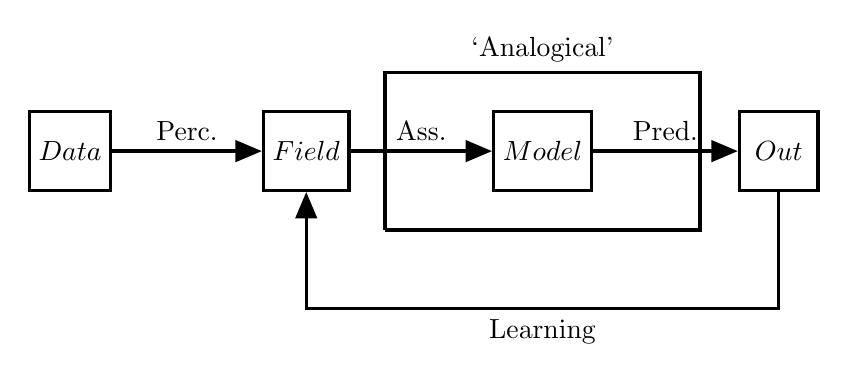
\begin{tikzpicture}[node distance=2cm]
\draw[very thick] (2,-1) -- (6,-1) -- (6,1) -- (2,1) node[midway,above] {`Analogical'} -- (2,-1);
\node (data) at (-2,0) [draw,very thick,minimum width=1cm,minimum height=1cm] {$Data$};
\node (syst) at (1,0) [draw,very thick,minimum width=1cm,minimum height=1cm] {$Field$};
\node (model) at (4,0) [draw,very thick,minimum width=1cm,minimum height=1cm] {$Model$};
\node (out) at (7,0) [draw,very thick,minimum width=1cm,minimum height=1cm] {$Out$};

% arrows
\draw [->,very thick] (data) -- (syst) node[midway,above]  {Perc.};
\draw [->, very thick] (syst) -- (model) node[midway,above] {Ass.};
\draw [->, very thick] (model) -- (out) node[midway,above] {Pred.};
\draw [->, very thick] (out) -- (7,-2) -- (1,-2) node[midway,below] {Learning} -- (syst);

\end{tikzpicture}
\caption{What has been referred to as analogical cognition may variously include parts of an associative mechanism, a cognitive system's internal model, and the application of that model for predictions and higher-order reasoning.  }

\end{center}
\end{figure}


[\dots]


In some of the first publications concerning transfer learning, transfer in neural networks is conceptualized as using the learned weights of a network at the outset---either directly or by using them as modulators to create other weights.  See for example \citet{Pratt1991,Pratt1993}.  Weights from a hidden layer to the output layer have also been shown to transfer classification capacity by \citet[p. 322]{Sharkeyetal1993}.  Modern deep ANNs have abundant hidden-to-hidden layer weights as well, and these are generally what are pre-trained in transfer learning techniques.  The input and output layers can be adjusted, but the largest number of transferred parameters are in the hidden layers.

%\begin{quote}
%In terms of connectionist research, adaptive generalization can be identified with the process by which a set of weights developed during the learning of one task is adapted for use on a second (novel) task.  The starting point for the second task can therefore be one of experience; its initializing weights incorporate the knowledge gained during training on the first task.  The question here then is one of understanding \emph{when} knowledge can be transferred between nets: identifying the circumstances under which pre-training on one task will assist (or interfere) with the performance of a subsequent task.  \cite[p. 314]{Sharkeyetal1993}
%\end{quote}

%Currently, an entry level data scientist does not need to train a new ANN for every task she encounters.  

With \texttt{keras}, a deep learning library for the Python programming language created by \citet{Chollet2015keras}, there are pre-trained deep networks (\emph{models}) available to be downloaded and used.  Similarly with \texttt{pytorch}.  These models are essentially sets of weights of certain dimensions, which have been trained on paradigmatic sets of data.  As an example, for image recognition, there are a number of models to pick off the shelf which have been trained on the ImageNet dataset from  \citet{Dengetal2009}.  This is a large dataset of images, and the models already have `experience' classifying the images in  this set.  These pre-trained models are useful for experimenting on new image data sets, and for when the number of data samples available on the new classification task are small.  Transfer learning is also making progress in other areas, such as natural language processing (NLP) with LSTMs.  Notably \citet{Ruderetal2018} recently introduced a method called Universal Language Model Fine-tuning which ``enables robust inductive transfer learning for any NLP task, akin to fine-tuning ImageNet models''.  The field is evolving rapidly, and perhaps future methods will involve some automated code writing from more generally capable models as well.  For example, Microsoft is using exclusive access to the GPT-3 model developed by OpenAI \citep{OpenAI_GPT-3} to translate natural language into code.


\subsection{EXCERPT: Bayesian Transfer (w/ Roland Poellinger)}

In briefly discussing the possibility of embedding such non-causal links into causal Bayes net structures, Verma and Pearl acknowledge the usefulness of such hybrid models:

\begin{quote}
The ability to represent functional dependencies would be a powerful extension from the point of view of the designer. These dependencies may easily be represented by the introduction of deterministic nodes which would correspond to the deterministic variables. Graphs which contain deterministic nodes represent more information than d-separation is able to extract; but a simple extension of d-separation, called D-separation, is both sound and complete with respect to the input list under both probabilistic inference and graphoid inference.  \cite[p. 75]{VermaPearlCausalNetworks1988} %\\\medskip
%
%D-separation is very similar to d-separation, only differing in that a path is rendered inactive by a set of nodes $Z$ under D-separation just\\in case it would be inactive under d-separation plus the case when a node on the path [\dots] is determined by $Z$.\\\medskip
\end{quote}

Symmetrical inter-theoretical relations like analogies are in our view a paradigm case study to implement such an extension.  We thus propose to model analogy as a relation between strictly correlated variables. It is  a non-causal and non-directional relation constructed on top of a syntactic isomorphism (formalized as a 1-1 function) in an extensions of a Bayes net causal model. Such hybrid structures have been discussed in philosophy  \citep{Poellinger2012}, as well as statistics (e.g., as chain graphs in \cite{Lauritzen01}).  We can extend a standard causal model triple $M=\langle U, V, F\rangle$ to a quadruple $\mathpzc{K}=\langle U, V, F, C\rangle$, where $U$ is a set of exogenous variables, $V$ a set of endogenous variables, $F$ a set of functional causal mechanisms (cf.  \cite[def. 7.1.1, p. 203]{Pearl2000}). The extension, $C$, is a set of \emph{epistemic contours}: a set of 1-1 functions $i_{j,k}$ that take the value of some variable $V_j$ and assign the value $i_{j,k}(V_j)$ to some other variable $V_k$ in the pattern. Importantly, intervening on one of these entangled variables will not break the contour.

Contours possess the properties we want for our analog relations. Yet, embedding entangled variables of this kind in Bayesian networks precisely renders them non-Markovian.\footnote{When Pearl claims that ``[t]he Markovian assumption [\dots] is a matter of convention, to distinguish complete from incomplete models''(Cf. \citep[p. 61]{Pearl2000} he naturally has Bayes net causal models (with distinct variables) in mind, which we just dismissed.} In the general case, the inferential framework must be tweaked to retain soundness,\footnote{For consistent reasoning and efficient computation of causal knowledge patterns to remain possible at all, acyclicity, independence (as expressed in the graphical \emph{d}-separation criterion), and the \emph{identifiability of causal effects} receive new explications. \cite{Poellinger2012} introduces a further graphical criterion, the \emph{principle of explanatory dominance}, to define under which conditions the Markov requirement can be reclaimed and extended Bayes nets can be utilized for causal inference.  
%Structure alone does not suffice for this task---more information is needed and comes in the form of intensional defaults and deviants as discussed, e.g., by Christopher \citet{Hitchcock2007}.
% By way of modifying the concept of \emph{identifiability of causal effects} it can be stated in which contexts which sub-portions of a partially directed graph support causal inference.
} but in our special case with a single intertheoretical bridge, we only require the idea of utilizing an undirected functional link to join two probabilistic chains (i.e., our two frames). So, how can we spell out analogical inference across this newly introduced bridge?

%Model nodes furthermore have an inner structure, where elements can be mapped onto each other in a unique way.  This means that on a more abstract level there is a one-one mapping between variables.
%[REF PEARL FUNCTIONAL RELATION FROM ROLAND's DISSERTATION]
%[QUICK INTRO TO CONTOURS MATH]



%\subsection{Analogical inference across symmetric links}\label{sec:application}

%In contrast to the general outline of epistemic contours above, analog contours are not generally transitive.  Thus, EC cliques will not be transitively closed.  [RIGHT?]  Just because $A::B$ and $B::C$ does not mean $A::C$.  Furthermore, we would not expect the same degree of confirmation to flow through such an informational link, although non-zero confirmation seems plausible enough to occur under certain circumstances.  That is, analogical contours will in general not fulfill these criteria, although there may be special cases that do.

In our proposal, the model-external postulate (or assumption, or also perception) ``$B_Q$ is similar to $B_F$ (in certain known respects)'' prompts the inclusion of a translation relation rather than the insertion of a new node. Analogical reasoning begins with a domain comparison which we characterize as the insertion of an inter-theoretical bridge.\footnote{This insertion can formally be understood as a structural mapping by which two frames are related.} Figure \ref{fig:SystemLadder} is a rendition of the Casimir effect example discussed above with the contour $i$ marking the analogical relationship between the frames at the level of systems $B_Q$ and $B_F$.

%\footnote{From now on we will omit the $\mathit{Aux}$ contributions in graphs, although the thorough reader may wish to keep them in mind.}

%\input{casimir-contour}

\begin{figure} [ht!]
\begin{center}
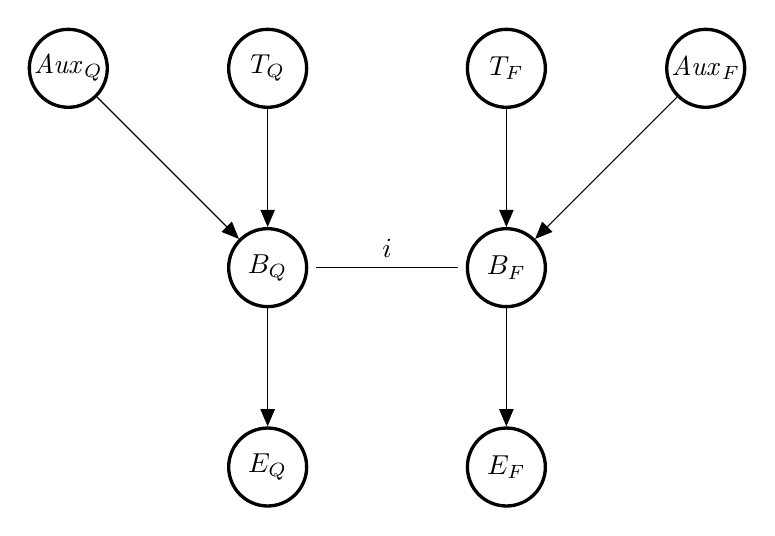
\begin{tikzpicture}[auto, node distance=5mm,
    latent/.style={circle,draw,very thick,inner sep=0mm,minimum size=10mm,align=center}]

\node[scale=0.99, latent] (X1) {$T_Q$};
\node[scale=0.99, latent, below=15mm of X1] (A) {$B_Q$};
\node[scale=0.99, latent, right=20mm of A] (B) {$B_F$};
\node[scale=0.99, latent, above=15mm of B] (X2) {$T_F$};
\node[scale=0.99, latent, below=15mm of A] (Y1) {$E_Q$};
\node[scale=0.99, latent, left=15mm of X1] (AUX1) {$\mathit{Aux}_Q$};
\node[scale=0.99, latent, right=15mm of X2] (AUX2) {$\mathit{Aux}_F$};
\node[scale=0.99, latent, below=15mm of B] (Y2) {$E_F$};
    \edge {X1} {A};
    \edge {X2} {B};
    \path[-,shorten >=1mm,shorten <=1mm] (A) edge node[midway]{$i$} (B);
    \edge {B} {Y2};
    \edge {A} {Y1};
    \edge {AUX1} {A};
    \edge {AUX2} {B};

 
\end{tikzpicture}
\caption{System-level analogy as epistemic contour $i$ with the intertheoretical bridge $i$ between $B_Q$ and $B_F$.}
\label{fig:SystemLadder}
\end{center}
\end{figure}












In this graph, the undirected edge between $B_Q$ and $B_F$, along with the formal explication we have introduced, provides a means for implementing analog confirmation as we have construed it.  A scientist or an artificial system can obtain $P(T_Q\,|\,E_F)>P(T_Q)$ while retaining the information represented by the undirected edge, and the ability at some later time to provide confirmation for $T_F$.  While in this case we might not need or want to confirm $T_F$, a general account \emph{should} provide for this.

One might wish to instead represent the analogical contour between $T_Q$ and $T_F$ (Figure \ref{fig:SystemLadder(STRONG)}).  However, this would be a much stronger claim since $B_Q$ and $B_F$ are determined to an additional extent by auxiliaries.  After all, confirmatory boosts in probability may be divided between the theory and auxiliary assumptions as per the Duhem-Quine problem.  An analogy at the theory level is, in some sense, an analogy that could be a step further towards unification than one at the system level.  

%We will return to briefly discuss (pre-)unification in Sec.\ \ref{sec:pre-unification}.

%\input{casimir-contour-strong}
\begin{figure} [ht!]
\begin{center}
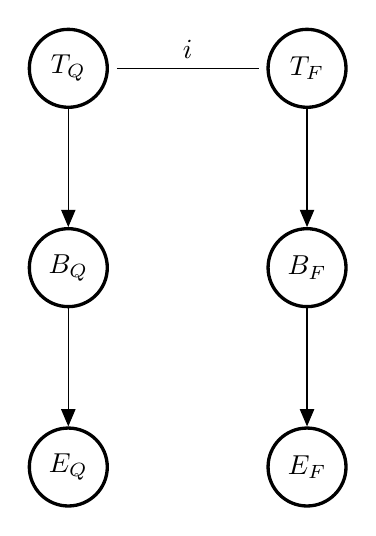
\begin{tikzpicture}[auto, node distance=5mm,
    latent/.style={circle,draw,very thick,inner sep=0mm,minimum size=10mm,align=center}]

\node[scale=0.99, latent] (X1) {$T_Q$};
\node[scale=0.99, latent, below=15mm of X1] (A) {$B_Q$};
\node[scale=0.99, latent, right=20mm of A] (B) {$B_F$};
\node[scale=0.99, latent, above=15mm of B] (X2) {$T_F$};
\node[scale=0.99, latent, below=15mm of A] (Y1) {$E_Q$};
\node[scale=0.99, latent, below=15mm of B] (Y2) {$E_F$};
    \edge {X1} {A};
    \edge {X2} {B};
    \path[-,shorten >=1mm,shorten <=1mm] (X1) edge node[midway]{$i$} (X2);
    \edge {B} {Y2};
    \edge {A} {Y1};

 
\end{tikzpicture}
\caption{Theory-level analogy as epistemic contour $i$ with the intertheoretical bridge $i$ between $T_Q$ and $T_F$.}
\label{fig:SystemLadder(STRONG)}
\end{center}
\end{figure}





















A potential option would also be to insert a collider structure between the model (system) levels representing an analogy.  However, as we have argued, granted analogies should not be represented as a node.  It is unclear what the content of the node would be, and the values it could take would arguably  depend upon a meta-level analysis of the network (i.e., it would be a self-referential node).  We think our approach of modeling the analogy as a functional relation is more consistent with the case study, as well as mathematically useful for future applications of the method.  Furthermore, there is support from the cognitive science literature treating analogy as an associative perceptual mechanism (i.e. structure mapping).  In this way, the transfer of knowledge from one domain to the other is \emph{direct}, not necessarily the result of a top-down generalization.  

%\marginal{Go through all possible ways of confirmation across c?}
%\marginal{collider would do it, but what is the content of the node? can only be meta-property of the network! should be relation.}

%emphasize that analogy is a structural transformation:
%
%Talk about relevance filter, sub-iso, analogy as structural transformation (based on meega)  vs node insertion, and confirmation across a theoretical bridge (not via switch node); remember Mark Colyvan's morphism through zigzag translation (as a process towards isomorphism!?) %Use Godehard Link, CoLo pp. 398 ff.

%\subsection{Translation via relevant sub-isomorphisms}\label{sec:sub-iso}

We take analog contours to be an expression of a modeling relationship between frameworks.  It can be thought of formally as a translation relation based on a \emph{relevant sub-isomorphism}, which has been anticipated in the literature on models and representations in science, cf.\ \cite{SEP2012}:

%\footnote{We have included in our bibliography the complete references cited in this quote for completeness.}

\begin{quote}
%Although this question is not explicitly addressed in the literature on the so-called semantic view of theories, some answers seem to emerge from its understanding of models. 

One version of the semantic view, one that builds on a mathematical notion of models, posits that a model and its target have to be isomorphic (van \cite{vanFraassen1980}; \cite{Suppes2002}) or partially isomorphic (Da \cite{DaCostaetal2003}) to each other. Formal requirements weaker than these have been discussed by \cite{Mundy1986} and \cite{Swoyer1991}. Another version of the semantic view drops formal requirements in favor of similarity (\cite{Giere1988,Giere2004}; \cite{Teller2001}). This approach enjoys the advantage over the isomorphism view that it is less restrictive and also can account for cases of inexact and simplifying models. However, as Giere points out, this account remains empty as long as no relevant respects and degrees of similarity are specified. The specification of such respects and degrees depends on the problem at hand and the larger scientific context and cannot be made on the basis of purely philosophical considerations (\cite{Teller2001}).
\end{quote}

\nocite{vanFraassen1980}
\nocite{Suppes2002}
\nocite{DaCostaetal2003}
\nocite{Mundy1986}
\nocite{Swoyer1991}
\nocite{Giere1988}
\nocite{Giere2004}
\nocite{Teller2001}


We follow this line of reasoning and formulate a relevance filter in order to capture the purpose-driven selection of theoretical entities to be translated. Of course, basing analogy on a purpose-driven relevance concept makes the concept of analog models context-specific.  The important point is that there is \emph{some} structural relationship which is mapped between the model and target systems.  We can embrace this and call $B_F$ an analog model of $B_Q$ \emph{relative to}

\begin{enumerate}
\item a relevance filter $Rlv$;
\item a bijection between the relevant properties of $B_Q$ and $B_F$ (an isomorphism between sub-structures of $B_Q$ and $B_F$).
\end{enumerate} 

The filter function $Rlv$, an indicator function over the descriptive elements of both frameworks, selects for each semantic category (for individual objects and each set of n-ary relations between such objects) subsets of equal magnitude; i.e., for each category:

\begin{equation}
||\,Rlv(B_Q)\,|| = ||\,Rlv(B_F)\,||\,.
\end{equation}

%For relevant properties $P$ and object vectors $\mathbf{x}$ of a given framework, the translation function (or: interpretation) $i$ bijectively translates objects and sets of objects into a second framework; for $P_Q = i(P_F)$ and $\mathbf{x}_Q = i(\mathbf{x}_F)$:

If $B_Q$ and $B_F$ behave alike with respect to relevant parts (i.e., parts selected by $Rlv$) that are described by $P_Q \mathbf(x)_Q$ and $P_F \mathbf(x)_F$ (with properties $P$ of objects $x$ in the respective models), then the following formula explicates the analog relation between frameworks via translation $i$:

\begin{equation}
\forall P_F, \mathbf{x}_F (P_F(\mathbf{x}_F) \leftrightarrow P_Q(\mathbf{x}_Q) )\,.
\end{equation}

Note that this isomorphism might be the result of iteratively fine-tuning non-bijective translations between the frameworks.%\footnote{We are thankful to Mark Colyvan for valuable discussions about the nature of this morphism.}

Having defined the propagation of information across the epistemic contour in this way, tracing confirmatory support in Fig.\ \ref{fig:SystemLadder} yields the following:
\begin{eqnarray}
P(B_F \,|\, E_F ) > P(B_F)\label{eq:fluidEvidence}\\
P(T_Q \,|\, B_Q ) > P(T_Q)\label{eq:quantumSystem}\\
P(i(B_F) \,|\, B_F ) > P(i(B_F))\label{eq:contour}
%\item $P(B' | T_Q ) > P( B' )$
%\item $P(T_{Q} | B' ) > P( T_{Q} )$
\end{eqnarray}
where $i(B_F)$ represents specific information about the properties of $B_Q$ relevant for the analogical inference (i.e., as chosen by the filter function). Eq.\ \ref{eq:contour} exploits the characterization of contour $i$ as 1-1 function: Learning $B_F$ tells us more about the $Rlv$-selected properties and objects at the core of $B_Q$, thereby raising our degree of belief in those $B_Q$ that are compatible with $i(B_F)$. Now, by transitivity, \ref{eq:fluidEvidence}, \ref{eq:quantumSystem}, and \ref{eq:contour} together entail
\begin{equation}
P(T_Q \,|\, E_F ) > P(T_Q),\label{eq:contourconfirmation}
\end{equation}
which was implied by our list of desiderata above.  Formula \ref{eq:contourconfirmation} is an instance of Bayesian confirmation---this time across theoretical frameworks, though, and it encodes what we set out to achieve: Bayesian confirmation from an analog model.

%\footnote{As soon as one learns of a specific instantiation of $i(B_F)$, i.e., the relevant core of $B_Q$, those theoretical entities not in the $Rlv$ mapping must be updated in line with consistency requirements.}


\section{Deep Learning Internship at Cray, Inc.}

\noindent Cray, now part of Hewlett Packard Enterprise,  manufactures supercomputers (putting together racks, cabinets, interconnects). They also provide high performance software to help customers like national scientific labs deploy jobs onto petascale and exascale compute clusters. \\

\noindent I worked with Cray's Distributed Deep Learning Plugin team. The plugin is a simple wrapper to modify python machine learning scripts to work across GPU clusters, using Message Passing Interface (MPI) (e.g. AllReduce) to communicate gradients between threads and average them.  I applied, tested, and experimented with the Plugin across multiple GPUs (gradient averaging using MPI), on a variety of ANN architectures including: LSTM, CNN, CapsNet, and Deep RL/DQN.  The latter was the most sophisticated, and should have been prioritized since I ended up running out of time in the internship before the plugin was functional on a deep reinforcement learning model. \\

\noindent \textbf{What I Used:} Python, Jupyter, Slurm, SSH onto \faLinux \  Linux GPU clusters, Keras, Anaconda, Bash, Git.  I mainly used Keras, scheduled jobs via Slurm, managed ML/DL packages and versions with Anaconda and pip, and committed code to internal git repos. \\

\noindent \textbf{What I Learned:}  Parallelization through distributing computation to threads and communicating between them (MPI).  Initiation task on day 1 was to estimate the value of $\pi$ with a parallelized Monte Carlo simulation in Fortran.  Distinction between Model and Data Parallelism.  \\

\noindent \textbf{Example Code Repo:} \href{https://github.com/CameronBeebe/Monte_Carlo}{Monte Carlo calculating pi with MPI and pyspark}







\section{Project: RL in Agent Based Modeling (Netlogo)}

Coding project in agent based modeling course at the MCMP using the Netlogo programming language.  I modified a simple reinforcement learning agent-based model to include a mechanism of ``forgetting''.  Years later I would describe the project as  utilizing a form of dropout. \\

\noindent \textbf{What I Learned:} Polya Urn as simple model of Reinforcement Learning (changing probability distribution of ``balls'' (actions) in an urn).  Noise as a regularizer. \\

\noindent \textbf{Full Paper:} \href{https://www.researchgate.net/publication/321228909_Modeling_Memory_in_Signaling_Games_Deep_and_Surface_Forgetting}{Modeling Memory in Signaling Games: Deep and Surface Forgetting}







\section{Academic environment and relevant courses}

Most courses I took involved some math, programming, and formal methods to varying degrees at LMU and through the Munich Center for Mathematical Philosophy (MCMP) and Graduate School of Systemic Neurosciences (GSN).  \\

\noindent The philosophy curriculum at the MCMP required basic formal methods: probability theory, information theory, formal logic, and basic linear algebra and calculus if working in more technical areas in philosophy of physics and interdisciplinary AI theory.  \\

\noindent Formal epistemology, rationality, and other philosophical aspects of cognition in consideration of artificial systems. \\

%\noindent Some of the courses included: \\

%Weekly Neurophilosophy seminars, Machine Epistemology (Wheeler), Rationality (Roy), The Unity and Plurality of Cognitive Science, Statistical Modeling and Data Analysis (Leibold), Philosophy of Probability (Mayo-Wilson), Quantum Information and Entanglement (Paredes), Philosophy of Quantum Computation (Cuffaro)\dots


\section{Coding}

I have the most experience with python and associated packages and tools.  I have used jupyter notebooks, pandas, scikit-learn, keras (and some tensorflow through tf.keras), and other related packages.  Before I got into python I also used Netlogo (a language specialized for agent based modeling and visualization), some octave and matlab, and I am comfortable working through the command line on linux/unix terminals.  In general, I am able to read and write code and learn new syntax.  

\section{Real World Data Experience}

For the last year and a half I have been working at a cultivation facility start up in Nederland, Colorado.  As we are a small team, most of us do everything.

\begin{multicols}{2}
\begin{itemize}
    \item \textbf{Measurement and Recording}: PH; total dissolved solids (tds) or parts per million (ppm); water temperature; room humidity and temperatures; nutrient solution amounts; plant waste weight; 
    \item \textbf{Calibration}: PH and TDS measurement devices.
    \item \textbf{Analysis:} We get reports of endogenous chemical composition in crop yields as tested by authorized labs, as well as reports of pesticide and spore residue (which must be below legal thresholds for sale).
\end{itemize}
\end{multicols}

\section{Other Experience}

\begin{multicols}{2}
\begin{itemize}
\item PyData talk on Transfer Learning
\item Nano degree Deep Learning (Udacity)
\item Talk at HLRS Stuttgart on Ashby's Cybernetics and characterizing ANNs as cybernetic regulators.
\item ML Reading Group attendance MCMP 2022 (Dr. Sterkenberg)
\item Talk about ChatGPT at local library in Nederland, CO.
\end{itemize}
\end{multicols}

\bibliographystyle{apacite}
\bibliography{MyBibliography1}


\end{document}  